\documentclass[letterpaper, 10 pt, conference]{ieeeconf}
\overrideIEEEmargins

% The following packages can be found on http:\\www.ctan.org
\usepackage{graphics} % for pdf, bitmapped graphics files
\usepackage{epsfig} % for postscript graphics files
\usepackage{mathptmx} % assumes new font selection scheme installed
\usepackage{times} % assumes new font selection scheme installed
\usepackage{amsmath} % assumes amsmath package installed
\usepackage{amssymb} % assumes amsmath package installed
\usepackage[activate={true,nocompatibility},final,tracking=true,kerning=true,spacing=true,factor=1100,stretch=10,shrink=10]{microtype} % nicer typesetting

\usepackage{array}
\newcolumntype{C}{>{$}c<{$}}

\title{\LARGE \bf Portfolio Optimization Based on a Complex Networks Model\\
  \normalsize TODO: propose a better title}

\author{Lovre Mr\v{c}ela et al.}

\begin{document}

  \maketitle
  \thispagestyle{empty}
  \pagestyle{empty}
    
  \begin{abstract}
    
  A new algorithm for portfolio optimization is presented which is based on statistical arbitrage, with potential method used to obtain the most preferred assets.
  A graph that represents preference relations among financial assets (i.e., if an edge exists going from asset A to asset B, then A is preferred over B) is constructed at each time step a, using the modified version of statistical arbitrage.
  Then, the preference flow of each asset is calculated, using the potential method\cite{caklovic}, from which the most preferred assets are selected into the portfolio for each time step.
  
  Method has been tested on dataset XY, and\dots (TODO: what happened)
  
  \end{abstract}
  
  \section{INTRODUCTION}
  
  The task of portfolio optimization is to try to enhance various criteria, which most of the time include maximization of expected return and minimization of deviation\dots
  
  The approach that is taken in this paper relies on finding abrupt deviations of price relations between in the observed set of assets.
  Algorithm works on pairs of assets, looking for such uncommon deviations, so generally it is expected to perform better where there is larger number of assets.
%  Each asset is compared to all other assets while looking for such specific deviations, so, in general, this algorithm performs better where there is larger number of assets.
  
  
%  Approach taken in this paper relies on statistical anomalies which are detected by observing past windows of time at each time step.
%  In this paper, approach was to create a portfolio using a large number of assets among which exist pairs that behave similarly during certain period.
%  At each time step, a past window of time is observed for finding pairs that abruptly stop behaving similarly.
  
  \section{KEY COMPONENTS}
  
  Following are the descriptions of two key components in the algorithm: graph of preference relations, and choosing assets for the portfolio...
  
  \subsection{Graph of preference relations}
  
  This is a graph whose vertices represent assets and edges represent how much more is one asset preferred over the other.
  An example is shown on the Fig. \ref{fig:graph}.
  The measure of this preference is determined by a statistical arbitrage algorithm, and it corresponds to the magnitude of two assets' price ratio going out of what is statistically considered `normal' range.
  This is illustrated on Fig. \ref{fig:devmag}.
  
  \begin{figure}[htb]
    \centering
    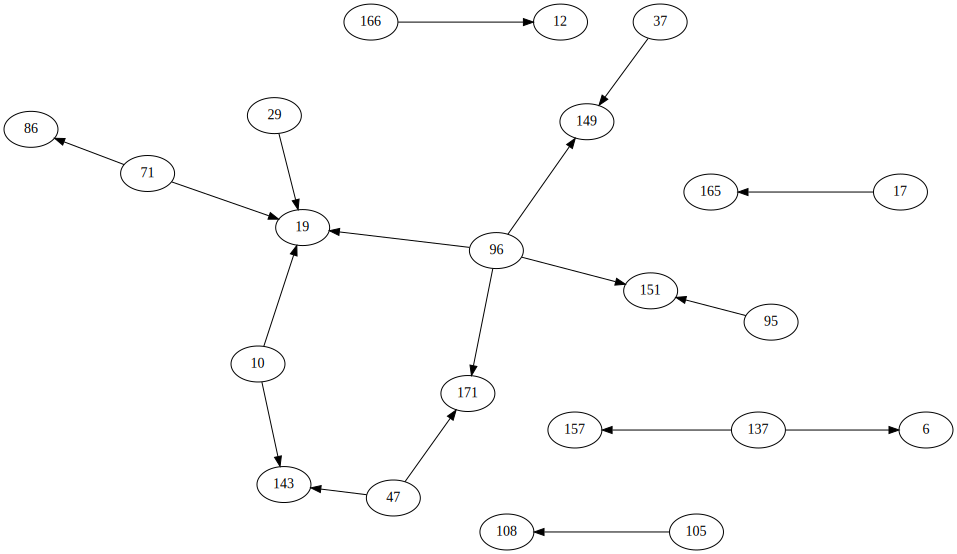
\includegraphics[width=\columnwidth]{graphics/output_0573.pdf}
    \caption{TODO: put image with weights on edges}
    \label{fig:graph}
  \end{figure}
    
  \begin{figure}[htb]
    \centering
    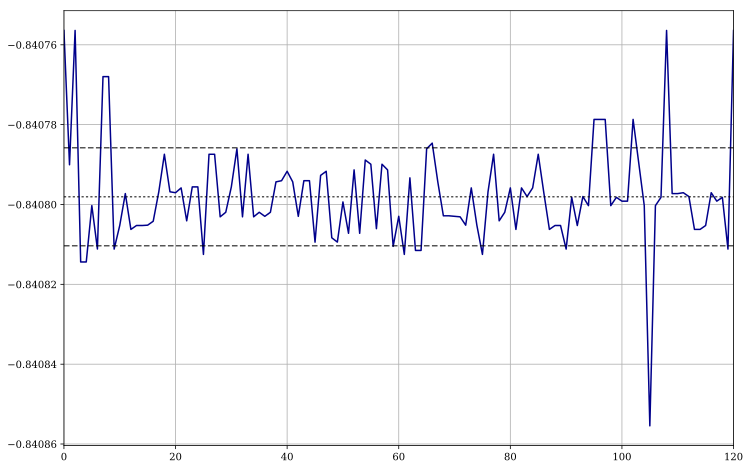
\includegraphics[width=0.9\columnwidth]{graphics/deviation-magnitude.png}
    \caption{TODO: put a better image, this is just for a placeholder}
    \label{fig:devmag}
  \end{figure}

  \subsection{Preference flow}
  
  \verb|TODO| 
  
  Include measure of inconsistency?
    
  \section{ALGORITHM} 
  
  Parameters of the algorithm are:
  \begin{itemize}
    \item $T$ - length of the past time window
    \item $\alpha$ - the deviation threshold
  \end{itemize}
  
  Let there be total of $N$ assets in $D$ days.
  Let price of asset $i$ at the time step $t$ be $a_i^{(t)}$, for $i \in 1..N$ and $t \in 0..D-1$.
  The log prices $b_i^{(t)}$, log price differences $c_{i,j}^{(t)}$ between assets $i$ and $j$, and rolling means $m_{i,j}^{(t)}$ and standard deviations $d_{i,j}^{(t)}$ of log price differences over past time window of size $T$ are obtained as follows:
  
  \begin{equation} b_i^{(t)} = \log\left(a_i^{(t)}\right), \end{equation}
  \begin{equation} c_{i,j}^{(t)} = b_i^{(t)} - b_j^{(t)}, \end{equation}
  \begin{equation} m_{i,j}^{(t)} = \frac{1}{T}\sum_{\tau=t-T+1}^{t} c_{i,j}^{(\tau)} \label{eq:m}, \end{equation}
  \begin{equation} d_{i,j}^{(t)} = \sqrt{\frac{1}{T}\sum_{\tau=t-T+1}^{t} \left(c_{i,j}^{(\tau)} - m_{i,j}^{(t)} \right)^2} \label{eq:d}. \end{equation}
  
  Note that calculating means and standard deviations of log price differences separately for each time step $t$ is rather computationally inefficient when dealing with rolling windows of data.
  Therefore, it is advisable to use a rolling algorithm as described in the appendix.
  On that note, $c_{i,j}^{(t)}$, $m_{i,j}^{(t)}$, and $d_{i,j}^{(t)}$ may be more efficiently stored contiguously in memory as a matrix, using following coding scheme: a pair $(i, j)$, where $i < j$, should be encoded to $k$ as:
  \begin{equation} k = N \cdot (i - 1) + j - 1 - \left. i \cdot (i + 1) \middle/ 2\right., \end{equation}
  and decoded from $k$ as:
  \begin{equation} i = \left\lfloor N + 1/2 - \sqrt{(N + 1/2)^2 - 2(N + k)} \right\rfloor, \end{equation}
  \begin{equation} j = k + i \cdot \left.(i + 1) \middle/ 2\right. - N \cdot (i - 1) + 1. \end{equation}
  An example of proposed coding is shown on figure \ref{fig:coding}.
  
  \begin{figure}[htb]
    \centering
    \begin{tabular}{C|CCCCC}
      i/j & 1 & 2 & 3 & 4 & 5 \\ \hline
      1 & \cdot & 0 & 1 & 2 & 3 \\
      2 & \cdot & \cdot & 4 & 5 & 6 \\
      3 & \cdot & \cdot & \cdot & 7 & 8 \\
      4 & \cdot & \cdot & \cdot & \cdot & 9 \\
      5 & \cdot & \cdot & \cdot & \cdot & \cdot
    \end{tabular}
    \hspace{0.8cm}
    \begin{tabular}{C|CC}
    k & i & j \\ \hline
    0 & 1 & 2 \\
    1 & 1 & 3 \\
    2 & 1 & 4 \\
    3 & 1 & 5 \\
    4 & 2 & 3 \\
    5 & 2 & 4 \\
    6 & 2 & 5 \\
    7 & 3 & 4 \\
    8 & 3 & 5 \\
    9 & 4 & 5 \\
    \end{tabular}
    \caption{Example of the proposed coding scheme, for $N = 5$. A dot $(\cdot)$ indicates that that combination is not used.}
    \label{fig:coding}
  \end{figure}
  
  \subsection{Creating the graph}
  
  Using the obtained $c_{i,j}^{(t)}$, $m_{i,j}^{(t)}$, and $d_{i,j}^{(t)}$ it is now possible to create a graph of preference relations between assets for each time step $t$.
  Considering the time step $t$, we find all such pairs of assets $(i,j)$ for which holds:
  
  \begin{equation}
    \label{eq:thresh}
    \left| c_{i,j}^{(t)} - m_{i,j}^{(t-1)} \right| > \alpha \cdot d_{i,j}^{(t - 1)},
  \end{equation}
  i.e. current log price difference is at least $\alpha$ deviations distant from mean value of the past time window.

  Afterwards, for each observed pair $(i,j)$ that breaks the threshold we add into graph vertices $i$ and $j$, and a weighed edge going from $i$ to $j$, with weight $w_{i,j}^{(t)}$ obtained as:
  
  \begin{equation}
    \label{eq:weight}
    w_{i,j}^{(t)} = \left. \left(c_{i,j}^{(t)} - m_{i,j}^{(t-1)}\right) \middle/ d_{i,j}^{(t-1)} \right..
  \end{equation}
  
  Thus, it is possible to create a relatively sparse graph for each time step $t \in T..D-1$.
  At some time steps it is possible that the graph could be empty, if it is the case that no pair $(i,j)$ satisfies (\ref{eq:thresh}).
  Lower values of parameter $\alpha$ yield denser graphs.
  
  \subsection{Choosing assets from graph}
  
  From previously obtained graph it is possible to tell which pair of assets has the highest preference flow.
  However it is not yet possible to directly tell which is the most preferrable asset, or obtain the measure of preference for individual assets.
  For this we need to calculate some sort of potential for each node in graph, which corresponds to difference in amount of flow going in and out of the node.
  A quick way to do this is by using the potential method as described in \cite{caklovic}.
  The summary of the method is as follows:
  \begin{enumerate}
    \item Let $\mathbf{A}$ be the incidence matrix of previously obtained graph. $\mathbf{A}$ has following properties:
    \begin{enumerate}
      \item each row corresponds to an edge in the graph, and each column to a node,
      \item for every edge in the graph going from node $i$ to node $j$, there is a corresponding row that has $-1$ and $1$ in columns that correspond to nodes $i$ and $j$, respectively,
      \item the remainder of elements in the matrix are zeros.
    \end{enumerate}
    \item Let $\mathbf{F}$ be column vector that contains edge weights, and order of the edges is consistent with order of the edges in $\mathbf{A}$.
    
    \item Let $\mathbf{X}$ be column vector that contains potentials of each node, and order of the nodes is consistent with order of the nodes in $\mathbf{A}$.
    
    \item Now $\mathbf{A}$, $\mathbf{X}$, and $\mathbf{F}$ should satisfy the equation
    \begin{equation}
      \label{eq:flowover}
      \mathbf{A} \mathbf{X} = \mathbf{F},
    \end{equation}
    meaning that the difference between potential of any two nodes should result result in weight of the edge between them.
    Most of the time this represents an overdetermined system since $\mathbf{A}$ has more rows than columns, so we convert it to a least squares problem:
    \begin{equation}
      \label{eq:flow}
      \begin{gathered}
      \min_{\mathbf{X}} \left\{ \left \lVert \mathbf{A} \mathbf{X} - \mathbf{F}\textsl{} \right \rVert ^ 2 \right\} \Rightarrow
      \frac{\partial}{\partial \mathbf{X}} \left \lVert \mathbf{A} \mathbf{X} - \mathbf{F}\textsl{} \right \rVert ^ 2 = \mathbf{0},
      \end{gathered}
    \end{equation}
    from which we obtain the equation:
    \begin{equation}
      \mathbf{A}^{T} \mathbf{A} \mathbf{X} = \mathbf{A}^{T} \mathbf{F}.
    \end{equation}
    Following constraint is also added:
    \begin{equation}
      \label{eq:sumiszero}
      \underbrace{\begin{bmatrix} 1 & 1 & \cdots & 1 \end{bmatrix}}_{N} \cdot \mathbf{X} = 0
    \end{equation}
    to ensure that total amounts of positive and negative potential are equal.
      
    \item Joining the previous two equations together by adding (\ref{eq:sumiszero}) to each row of (\ref{eq:flow}) results in:
    \begin{equation}
      \begin{aligned}
        \mathbf{A}^{T} \mathbf{A} \mathbf{X} + \mathbf{J} \mathbf{X} &= \mathbf{A}^{T} \mathbf{F}\\
        \left[\mathbf{A}^{T} \mathbf{A} + \mathbf{J} \right] \mathbf{X} &= \mathbf{A}^{T} \mathbf{F},
      \end{aligned}
    \end{equation}
    where $\mathbf{J}$ is a matrix of ones with same dimension as $\mathbf{A}^{T} \mathbf{A}$.
    Finally, solving for $\mathbf{X}$ gives us:
    \begin{equation}
      \mathbf{X} = \left[\mathbf{A}^T \mathbf{A} + \mathbf{J} \right]^{-1} \mathbf{A}^T \mathbf{F}.
    \end{equation}
  \end{enumerate}
      
  \section{RESULTS}
  
  \verb|TODO|

  \section{CONCLUSIONS}
  
  \verb|TODO|
    
  % \addtolength{\textheight}{-12cm} % This command serves to balance the column lengths
  % on the last page of the document manually. It shortens
  % the textheight of the last page by a suitable amount.
  % This command does not take effect until the next page
  % so it should come on the page before the last. Make
  % sure that you do not shorten the textheight too much.
  
  \section*{APPENDIX}
  
  \subsection{Rolling mean and variance algorithm}
  \label{sub:rolling}
  
  \verb|TODO|

  \begin{thebibliography}{9} % mind the label-width
    
  \bibitem{caklovic} L. \v{C}aklovi\'{c}, Decision Making by Potential Method
%    \bibitem{c2} W.-K. Chen, Linear Networks and Systems (Book style).	Belmont, CA: Wadsworth, 1993, pp. 123Ð135.
%    \bibitem{c3} H. Poor, An Introduction to Signal Detection and Estimation.   New York: Springer-Verlag, 1985, ch. 4.
%    \bibitem{c4} B. Smith, ÒAn approach to graphs of linear forms (Unpublished work style),Ó unpublished.
%    \bibitem{c5} E. H. Miller, ÒA note on reflector arrays (Periodical styleÑAccepted for publication),Ó IEEE Trans. Antennas Propagat., to be publised.
%    \bibitem{c6} J. Wang, ÒFundamentals of erbium-doped fiber amplifiers arrays (Periodical styleÑSubmitted for publication),Ó IEEE J. Quantum Electron., submitted for publication.
%    \bibitem{c7} C. J. Kaufman, Rocky Mountain Research Lab., Boulder, CO, private communication, May 1995.
%    \bibitem{c8} Y. Yorozu, M. Hirano, K. Oka, and Y. Tagawa, ÒElectron spectroscopy studies on magneto-optical media and plastic substrate interfaces(Translation Journals style),Ó IEEE Transl. J. Magn.Jpn., vol. 2, Aug. 1987, pp. 740Ð741 [Dig. 9th Annu. Conf. Magnetics Japan, 1982, p. 301].
%    \bibitem{c9} M. Young, The Techincal Writers Handbook.  Mill Valley, CA: University Science, 1989.
%    \bibitem{c10} J. U. Duncombe, ÒInfrared navigationÑPart I: An assessment of feasibility (Periodical style),Ó IEEE Trans. Electron Devices, vol. ED-11, pp. 34Ð39, Jan. 1959.
%    \bibitem{c11} S. Chen, B. Mulgrew, and P. M. Grant, ÒA clustering technique for digital communications channel equalization using radial basis function networks,Ó IEEE Trans. Neural Networks, vol. 4, pp. 570Ð578, July 1993.
%    \bibitem{c12} R. W. Lucky, ÒAutomatic equalization for digital communication,Ó Bell Syst. Tech. J., vol. 44, no. 4, pp. 547Ð588, Apr. 1965.
%    \bibitem{c13} S. P. Bingulac, ÒOn the compatibility of adaptive controllers (Published Conference Proceedings style),Ó in Proc. 4th Annu. Allerton Conf. Circuits and Systems Theory, New York, 1994, pp. 8Ð16.
%    \bibitem{c14} G. R. Faulhaber, ÒDesign of service systems with priority reservation,Ó in Conf. Rec. 1995 IEEE Int. Conf. Communications, pp. 3Ð8.
%    \bibitem{c15} W. D. Doyle, ÒMagnetization reversal in films with biaxial anisotropy,Ó in 1987 Proc. INTERMAG Conf., pp. 2.2-1Ð2.2-6.
%    \bibitem{c16} G. W. Juette and L. E. Zeffanella, ÒRadio noise currents n short sections on bundle conductors (Presented Conference Paper style),Ó presented at the IEEE Summer power Meeting, Dallas, TX, June 22Ð27, 1990, Paper 90 SM 690-0 PWRS.
%    \bibitem{c17} J. G. Kreifeldt, ÒAn analysis of surface-detected EMG as an amplitude-modulated noise,Ó presented at the 1989 Int. Conf. Medicine and Biological Engineering, Chicago, IL.
%    \bibitem{c18} J. Williams, ÒNarrow-band analyzer (Thesis or Dissertation style),Ó Ph.D. dissertation, Dept. Elect. Eng., Harvard Univ., Cambridge, MA, 1993. 
%    \bibitem{c19} N. Kawasaki, ÒParametric study of thermal and chemical nonequilibrium nozzle flow,Ó M.S. thesis, Dept. Electron. Eng., Osaka Univ., Osaka, Japan, 1993.
%    \bibitem{c20} J. P. Wilkinson, ÒNonlinear resonant circuit devicesize (Patent style),Ó U.S. Patent 3 624 12, July 16, 1990. 

  \end{thebibliography}
\end{document}
